
\subsection{Historical background}

\begin{frame}

\frametitle{The Aristotelian causal theory}

Although the Aristotelian paradigm was abandoned with the advent of modern science, the recovery of the distinction between material and formal cause was crucial for the development of the concept of \href{http://en.wikipedia.org/wiki/Closure_(mathematics)}{closure} applied to efficient causality in autonomous living systems.

	
\begin{center}
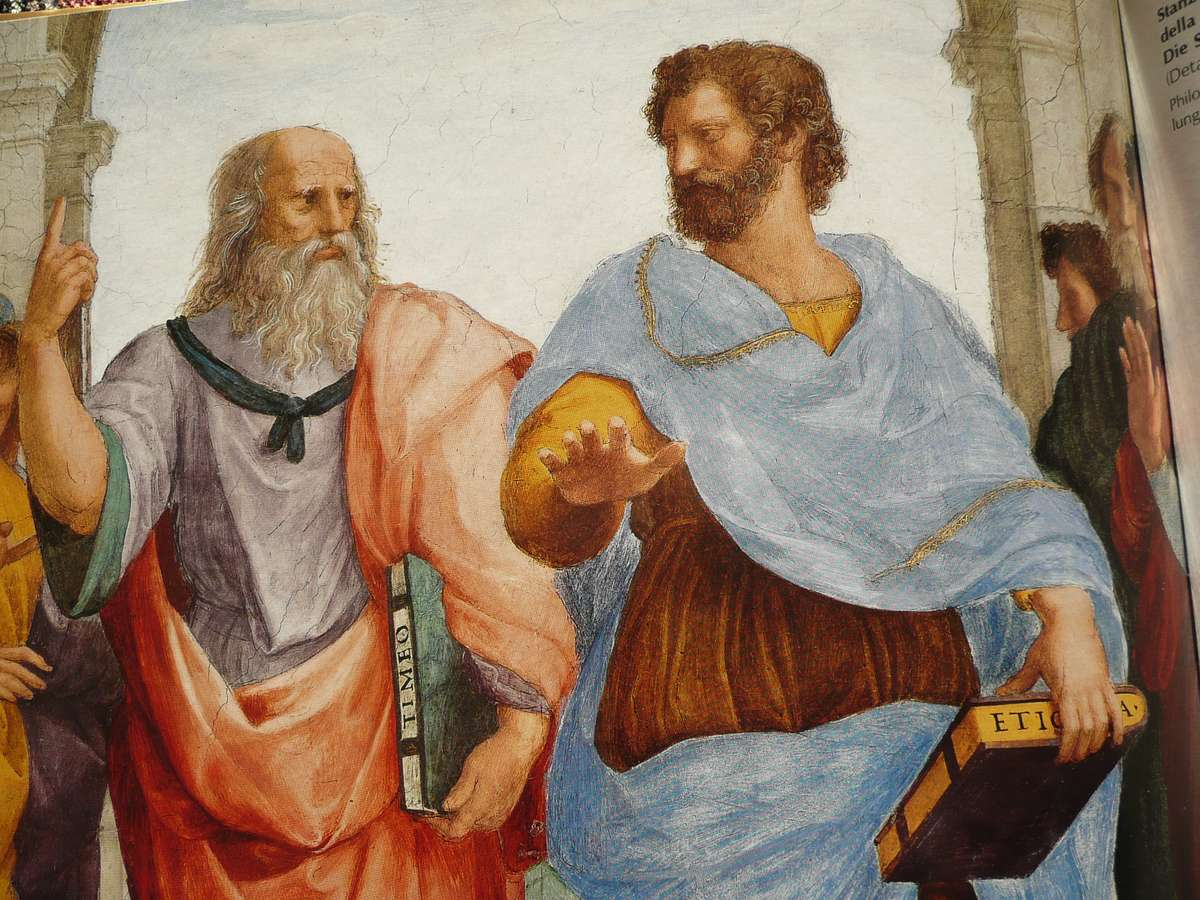
\includegraphics[width=3 cm]{fig/aristotle.jpg}

\end{center}
The four types of causes, according to Aristotle:	
 \begin{itemize}
  \item The \textbf{material cause} or stuff
  \item The \textbf{efficient cause} or force
  \item The \textbf{formal cause} or shape
  \item The \textbf{final cause} or aim
  \end{itemize}
\end{frame}



\begin{frame}

\frametitle{Rosen}

One of the most fertile attempts to capture the fundamental properties of biological systems is the work of Robert Rosen, who recovered the Aristotelian material cause and used category theory to shed some light on the problematic conceptualization of a living system as such. \cite{Rashevsky1954,Rosen1958a,Rosen1958,Rashevsky1965,Rosen1978,Rosen1985,Rosen1991}
 \begin{columns}
    \begin{column}{0.5\textwidth}
      \centering
		
\includegraphics[width=3 cm]{fig/rosen.jpg}
    \end{column}
    \begin{column}{0.5\textwidth}
      \centering
	      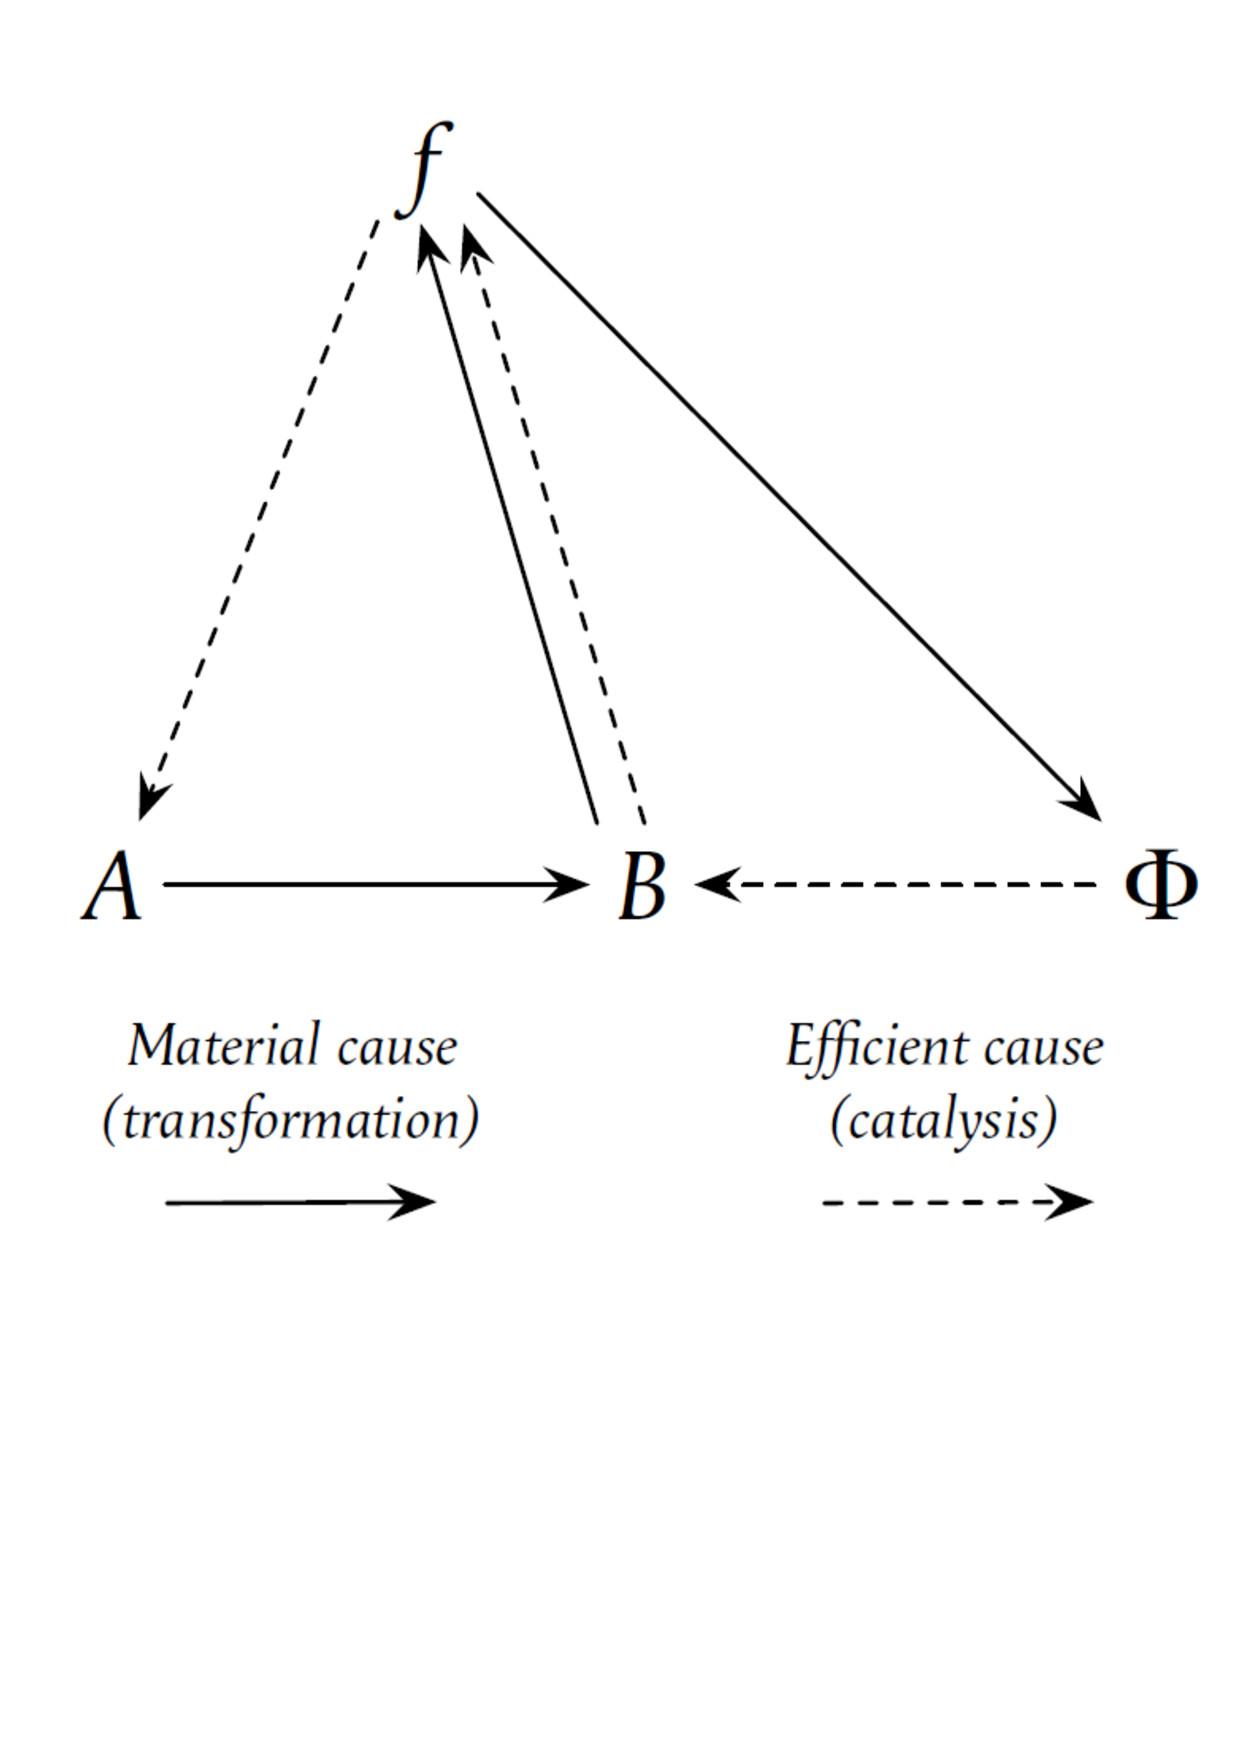
\includegraphics[width=4 cm]{fig/rosen_diagram.pdf}
    \end{column}
\end{columns}

\end{frame}

\begin{frame}

\subsection{MR systems}
\frametitle{Metabolism-Repair systems}
A metabolic mapping in a living system $\mathcal{L}$ can be thought as a morphism between two objects of the \textbf{category} $\mathcal{L}$ such that:
\begin{block}{metabolic function}
\begin{center}
	$\xymatrix@1{
	A\ar[r]^-{f} & B
	}$
\end{center}
\end{block}
As a first approximation, we can think of both objects as sets. Where $A$ represents the input metabolites and $B$  products of metabolic transformations.
\end{frame}

\begin{frame}
\frametitle{Metabolism-Repair systems}
\begin{itemize}
\item We can define all \textbf{metabolisms} together as the set of all the different morphisms between these objects referred to as $Hom(A,B)$. 
\item Metabolic enzymes decay, so they must be repaired, from the metabolic products, or the system comprised of them will disintegrate. 
\item Environmental fluctuations in $A$ have to be corrected by the differential availability and performance of the metabolic function.
\end{itemize}	
\end{frame}

\begin{frame}

\frametitle{Metabolism-Repair systems}
\begin{itemize}
\item Hence, there must be a collection of morphisms from $B$ to $Hom(A,B)$, also written as $B^A$, which can be identified with a \textbf{repair} system. So we have:

\begin{block}{metabolism, repair function}
\begin{center}
	$
	\xymatrix@1{
	A\ar[r]^f &B\ar[r]^-g & B^A}
	$
\end{center}
\end{block}
\item The repair system itself or $g \in B^{A^B}$ \footnote{this is notation for $Hom(B,Hom(A,B))$} also has a finite lifetime and needs to be {\it repaired} by some other system. 
\item This argument appears to fall into infinite regress, but a detailed analysis shows that a \textbf{replication} function that closes the system to efficient causation is implicit.
\end{itemize}
\end{frame}

\begin{frame}
\frametitle{infinite regress}
%	$$
%	\xymatrix@1{
%	A \ar[r]^{B^A}="ba" & B \ar@(r,ur)_(.5) {B^{A^B}} [];"ba"}
%	$$
%\begin{block}
	\begin{center}
		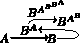
\includegraphics[width=0.4\textwidth]{fig/mrcatclose.pdf}
	\end{center}
%\end{block}
\end{frame}


\begin{frame}
\frametitle{infinite regress}
	\begin{center}
		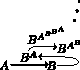
\includegraphics[width=0.4\textwidth]{fig/mrcatinf.pdf}
	\end{center}
\end{frame}

\subsection{hom-tensor adjunction}
\begin{frame}
\frametitle{hom-tensor adjunction}
Now let us consider that the category $\mathcal{L}$ is concrete and has products:
\begin{block}{products in $\mathcal{L}$}
Let $A,B,C,D \in Ob(\mathcal{L})$ and $f,g \in Mor(\mathcal{L})$ where $f  \in Hom(A,B)$ and $g  \in Hom(C,D)$. If $\mathcal{L}$ has products, then $A \times C, B \times D \in Ob(\mathcal{L})$ as well and $f \times g \in Mor(\mathcal{L})$ where $f \times g \in Hom(A \times C ,B \times D)$.
\end{block}
\end{frame}

\begin{frame}
\frametitle{hom-tensor adjunction}
In order for  $\mathcal{L}$  to be closed to efficient causation every morphism must be in turn an object of the category. The existence of so-called {\it exponential objects} is associated with a special evaluation mapping:
\begin{block}{metabolism evaluation map}
\abovedisplayskip=0pt
\begin{align*}
e_f : B^A \times A &\longrightarrow B\\
(f,a) & \longmapsto f(a)
\end{align*}
\end{block}
\end{frame}

\begin{frame}
\frametitle{hom-tensor adjunction}
Then the repair system $B^{A^B}$ must have another evaluation map in $Mor(\mathcal{L})$:
\begin{block}{repair evaluation map}
\abovedisplayskip=0pt
\begin{align*}
	e_g: B^{A^B} \times B &\longrightarrow B^A\\
	                (g,b) & \longmapsto    g(b)
\end{align*}
\end{block}
Suppose we want to evaluate a morphism $g \in B^{A^B}$, denoting the evaluation map provisionally as $h: (g,b)\rightarrow g(b) $ we can curry it as $[H(g)](b)$ that is a function of $B$ thus being an element of $B^{A^B}$ so $H: B \rightarrow B^{A^B} $.
\end{frame}

\begin{frame}
\frametitle{replication}
We can functionally close the system via the \textbf{replication} map:
\begin{block}{replication map}
\abovedisplayskip=0pt
\begin{align*}
R: B^A & \longrightarrow B^{A^B}\\
f & \longmapsto R(f)
\end{align*}
\end{block}
 \begin{columns}
    \begin{column}{0.5\textwidth}
      \begin{block}{metabolism evaluation map}
		\abovedisplayskip=0pt
		\begin{align*}
		e_f : B^A \times A &\longrightarrow B\\
		(f,a) & \longmapsto f(a)
		\end{align*}
		\end{block}
    \end{column}
    \begin{column}{0.5\textwidth}
		\begin{block}{repair evaluation map}
			\abovedisplayskip=0pt
			\begin{align*}
			e_g: B^{A^B} \times B &\longrightarrow B^A\\
	    			            (g,b) & \longmapsto    g(b)
			\end{align*}
		\end{block}
    \end{column}
\end{columns}
\end{frame}

\begin{frame}
A set of \textbf{boundary conditions} must be satisfied in order to achieve closure.

\begin{columns}[t]
   \begin{column}{0.5\textwidth}
		\begin{block}{boundary conditions}
		\abovedisplayskip=0pt
			\begin{align*}
			f(a) &= b : B\\
			g(b) &= f : B^A\\
			R(f) &= g : B^{A^B}
			\end{align*}
		\end{block}
	\end{column}
	\begin{column}{0.5\textwidth}
		\begin{block}{MR diagram}
		\abovedisplayskip=0pt
		$$	\xymatrix@1{
			A \ar[r]^{B^A}="ba" & B \ar@(r,ur)_(.5) {B^{A^B}} [];"ba"}$$
		\end{block}
	\end{column}
\end{columns}
%	$$
%	\xymatrix@1{
%	A \ar[r]^{B^A}="ba" & B \ar@(r,ur)_(.5) {B^{A^B}} [];"ba"}
%	$$
\end{frame}